\section{Theoretical work}\label{sec:theory}

In this section we will present our theoretical work on exploring the group announcement operator in GAL. In doing this, we will be building on the definitions that were established and introduced in the previous section.

\subsection{Introduction}


Throughout the rest of this thesis, we will refer to the previous by the following definition: 
\begin{definition}[Models]\label{def:model}
	Given a group of agents $\ags$, and a set of propositions $\props$, a model M is a structure \model{} , where
	\begin{itemize}
		\item $\states$ is a set of states
		\item $\rels$ is a function from every agent $a \in \ags$ to $a$'s equivalence relation $\rels_a \subseteq \states\times\states$. 
		\item $\vals(p)$ is a valuation function that for every proposition $p \in \props$ returns the set of states where $p$ is true
	\end{itemize}
\end{definition}

We will also frequently use $\rels$ as $s\rels_a t$, where $a\in\ags$ to signal that agent $a$ is unable to distinguish between states $s$ and $t$. When we wish to highlight specific states in a model we will denote this by writing $(M,s)$ to specify that we are referring to state $s$ in the model $M$, commonly known as a pointed model. This is the form that we will use when we are discussing the properties of a state $s$ in the context of some model $M$. 

A simple practical example of an epistemic model could be us imagining someone that doesn't know whether or not it is raining outside. If we focus solely on whether or not it is in fact raining outside, we might denote this proposition as $p$, where $p = $``It is raining outside". Since this agent, $a$ does not know whether it is raining, this means that in their mind there must be at least two possible worlds, or states; one where $p$ is true, and one where $p$ is false and that $a$ is unable to tell these two states apart. If we label these states as $s_0$ and $s_1$, we end up with the following model shown in Figure \ref{fig:basicEM}, where we use $\neg p$ to signify that $p$ is not true in $(M,s_1)$
\todo{Fix this reference so it points to the correct figure}

\begin{figure}[h]
	\label{fig:basicEM}
	\caption{A basic model with two states}
	\centering
	\scalebox{1.9}{
		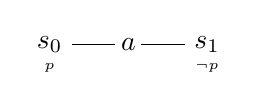
\begin{tikzpicture}[scale = 2.0, every label/.append style = {font=\tiny}]	
			\node[label={[label distance=-0.7cm]:$p$}] (s0) at (0,0) {$s_0$};
			\node[label={[label distance=-0.7cm]:$\neg p$}] (s1) at (1,0) {$s_1$};
		
			\path[every node/.append style={font=\fontsize{10}{0}, fill=white, inner sep=2pt}] 
				(s0) edge node {$a$} (s1);
		\end{tikzpicture}
	} %End scaling
	\break \textit{Note that since we are working with S5 models, all nodes (states) also have reflexive edges to themselves, even if they are not explicitly drawn in these figures}
\end{figure}

\subsection{Language and semantics}

Continuing with the model shown in Figure \ref{fig:basicEM}, we might want to express certain properties or verify that $p$ is indeed true in $(M,s_0)$, for this we would write $(M,s_0) \models p$, or that $s_0$ in the context of $M$ \textit{satisfies} $p$. More formally, $(M,s_0) \models p$ is true \textit{iff} $s_0 \in V(p)$ where if we go back to Definition \ref{def:model}, we can see that V is a valuation function for propositions, meaning that it returns the set of states in $M$, where $p$ is true. 

In general however, we might want to build more complex formulas to check against our models than simple propositions, for this we need connectives; and logics that define their semantics.

\begin{definition}[Group Announcement Logic] \hfill
	\label{def:GAL}
 	\begin{align*}
		\varphi ::= p \ | ~\neg\varphi ~|~ (\varphi~\wedge~\psi) ~|~ (\varphi~\vee~\psi) ~|~ \varphi 							\rightarrow \psi ~|~ K_a\varphi ~|~ [\varphi]\psi  ~|~ [G]\varphi
	\end{align*}
	Where $p$ is a proposition such that $p \in P$, $a$ is an agent i.e $a \in A$ and $G$ is a set of agents i.e $G \subseteq A$
\end{definition}

Definition \ref{def:GAL} defines the language of \lang{GAL} or more specifically, the set of legal formulas that can be built in accordance to GAL. It inductively specifies in BNF-notation how each operator in the language can be used to create new formulas. This notation however merely specifies the \textit{syntax} of the language, which ways we are allowed to arrange the symbols. In order to specify what each operator does, we also need semantics, which we will add through the satisfaction relation $\models$.

\begin{definition}[GAL Semantics] \hfill
	\label{def:GALsem}
	\begin{itemize}
		\item[] $\M,s \models p $ iff $ s \in \vals(p)$
		\item[] $\M,s \models \neg\varphi$ iff $ \M,s \not\models \varphi$
		\item[] $\M,s \models \varphi \wedge \psi $ iff $ \M,s \models \varphi $ and $ \M,s \models \psi$
		\item[] $\M,s \models \varphi \vee \psi $ iff $ \M,s \models \varphi $ or $ \M,s \models \psi$
		\item[] $\M,s \models \varphi \rightarrow \psi $ iff $ \M,s \not\models \varphi $ or $ \M,s \models \psi$
		\item[] $\M,s \models K_i\varphi $ iff for every $t$ such that $s\rels_{i}t$, $\M,s \models \varphi$
		\item[] $\M,s \models [\varphi]\psi $ iff $ \M,s \models \varphi $ implies that $ \M|\varphi,s \models \psi$
		\item[] $\M,s \models [G]\varphi $ iff for every set $\{\psi_i: i \in G\} \subseteq $ \lang{el}, $ \M,s \models [\bigwedge_{i\in G}K_i\psi_i]\varphi$ 
	\end{itemize}
\end{definition}

\todo{Mention tautologies and falsehoods, plus valid and satisfiable formulas ect}

Starting with the most basic component of our formulas we have propositions, commonly referred to as atoms or atomic formulas as propositions themselves are also formulas. If we want to check if some pointed model $\M,s \models p$ or satisfies some property $p$, then as we can see in Definition \ref{def:GALsem} we do this by seeing if the state $s$ is an element in the set of states where $p$ is true, more formally if $s \in \vals(p)$. 

For the explanation of our operators we will be using $\varphi$ and $\psi$ to represent arbitrary formulas. Negation, $\neg$ is relatively trivial, with $\neg\varphi$ simply meaning the negation of $\varphi$ and that $\M,s \models \neg\varphi$ if, and only if $\M,s \not\models\varphi$. Conjunction and disjunction, $\wedge$ and $\vee$ are also pretty simple, translating to `and' and `inclusive or', as can be seen from their definitions in Definition \ref{def:GALsem}. Implication, $\rightarrow$ can be somewhat loosely translated to `if $a$, then $b$', except if $a$ doesn't hold, then the implication automatically holds regardless of $b$. More specifically, the only time an implication is false is when $a$ is true and $b$ is false. We will also use $\varphi \leftrightarrow \psi$, to denote biimplications, meaning $(\varphi \rightarrow \psi) \wedge (\psi \rightarrow \varphi)$ throughout this thesis. 

The previous operators are all relatively basic and only express properties regarding the structures they are checked against, the remaining operators in our language are more interesting, as they also express properties regarding the knowledge of the agents in our systems shifting us towards epistemic logic. The $K_i$ operator is the first of these, with $\M ,s \models K_ap$ expressing that in our pointed model agent $a$ knows that the proposition $p$ is true. Verifying that this is the case however is where things get interesting, as the previous operators only express properties regarding single states, their scope is also limited to that single state, whereas the $K_i$ operator also requires us to check all the states that this agent is incapable of distinguishing from the current state. In order to check if $\M,s \models K_a\varphi$, we need to ascertain that all states a is unable to distinguish from s also satisfy $\varphi$. More specifically, that for all states $t\rels_as$, that $\M,t \models\varphi$. This is because if there exists any such state that does not satisfy $\varphi$, then agent $a$ considers it possible that $\varphi$ is not satisfied since they cannot tell if $t$ or $s$ is the actual state they are in.

While the $K_i$ operator lets us reason around the knowledge of our agents, the public announcement operator $[\varphi]\psi$ lets us update it, or at least add to it by informing the agents through a truthful announcement that some formula is true in the `current' state as defined by the pointed model we are checking the announcement in.
In Definition \ref{def:GALsem} we use the notation $\M|\varphi,s$ to denote $\M$ `updated' by $\varphi$, meaning $\M$ minus all states which do not satisfy $\varphi$.

\begin{definition}[Model Updates]
	\label{def:modupdate}
	$\M$ updated by $\varphi$ is defined as the following: $\M|_\varphi = \langle\states',\rels',\vals'\rangle$ where 
	\begin{align*}
			\states' &= \{s| s\in \states\textrm{ and }\M,s \models\varphi\} \\
			\rels_a' &= \rels_a \cap (\states' \times \states')~ \forall a\in A\\
			\vals'(p) &= \vals(p) \cap \states'~ \forall p \in P
	\end{align*}
\end{definition}

Informally, the definition above in Definition \ref{def:modupdate} can be read as filtering out all states in $\M$ which do not satisfy $\varphi$ and then constraining the equivalence relations for each agent and the valuation function to that filtered set of states.

The final and most interesting operator in \lang{GAL} is $[G]\varphi$, or the group announcement operator, where $G$ is some coalition of agents such that $G \subseteq \ags$. $\M,s \models [G]\varphi$ expresses that there is no way for the group $G$ to announce anything that can make $\varphi$ false in $\M,s$. Note however that the formulas the agents in $[G]$ can announce are constrained to basic epistemic formulas, or to \lang{el} as defined in Definition \ref{def:langel} in order to avoid making our definition of group announcements circular. \todo{Reword sentence} The syntax of $\{\psi_i: i\in G\}[\bigwedge_{i\in G}K_i\psi_i]\varphi$ intuitively means `the conjunction of all formulas $K_i\psi_i$ such that each agent $i$ knows their formula $\psi_i$ and that after this conjunction is announced, $\varphi$ is true'. As the definition in Definition \ref{def:GALsem} specifies that this has to hold for \textit{every} set of $\{\psi_i : i\in G\}$ however, it might be easier to think of it as there not existing a set such that $\M,s \not\models [\bigwedge_{i\in G}K_i\psi_i]\varphi$ or that $G$ does \textit{not} have the ability to prevent $\varphi$ from coming true.

\begin{definition}[Language of epistemic logic \lang{el}] \hfill
	\label{def:langel}
	\begin{itemize}
		\item[] $\M,s \models p $ iff $ s \in \vals(p)$
		\item[] $\M,s \models \neg\varphi$ iff $ \M,s \not\models \varphi$
		\item[] $\M,s \models \varphi \wedge \psi $ iff $ \M,s \models \varphi $ and $ \M,s \models \psi$
		\item[] $\M,s \models \varphi \vee \psi $ iff $ \M,s \models \varphi $ or $ \M,s \models \psi$
		\item[] $\M,s \models \varphi \rightarrow \psi $ iff $ \M,s \not\models \varphi $ or $ \M,s \models \psi$
		\item[] $\M,s \models K_i\varphi $ iff for every $t$ such that $s\rels_{i}t$, $\M,s \models \varphi$
	\end{itemize}
	Where all operators have their semantics defined as in Definition \ref{def:GALsem}
\end{definition}

We will also be using the duality of the two announcement operators, $\langle\varphi\rangle\psi$ and $\langle G\rangle\varphi$ which are defined as follows in Definition \ref{def:dual}.

\begin{definition}[Dual announcement operators] \hfill
	\label{def:dual}
	\begin{align*}
		\M,s &\models \dia{\varphi}\psi\textrm{ iff }\M,s \models \varphi\textrm{ and }\M|_\varphi,s \models \psi \\
		\M,s &\models \dia{G}\varphi \textrm{ iff there exists a set }\{\psi_i:i\in G\} \subseteq \textrm{\lang{el} such that: }\\
			   &\M,s \models \dia{\bigwedge_{i\in G}K_i\psi_i}\varphi
	\end{align*}

\end{definition}

The difference between $[\varphi]\psi$ and $\dia{\varphi}\psi$ is that the box notation `implies' that $\psi$ is true in the updated model, \todo{reword sentence} while the diamond notation requires both that $\M,s\models \varphi$ and $M|_\varphi \models \psi$ For group announcements, the box notation expresses that something has to hold after any possible set of announcements the coalition can make, while the dual $\dia{G}$ expresses that there exists at least one set of announcements for the agents in $G$ such that after their announcements $\varphi$ is true. An interesting observation to make is that like in modal logics we have the same relation between $[\psi]\varphi$ and $\dia{\psi}\varphi$ as $\square\varphi$ and $\lozenge\varphi$, namely that $[\psi]\varphi \leftrightarrow \neg\dia{\psi}\neg\varphi$

When we are discussing announcement operators we are usually also interested in the knowledge of the agents in our system, as such it is useful to be able to refer to the set of states an agent considers indistinguishable from the given state. For this we will be using the notion of equivalence classes, defined as the following:

\begin{definition}[Equivalence classes]
	\label{def:eqclass}
	Given a state $s$ and some agent $a$, a's equivalence class for $s$ is denoted by $\eqc{s}_a$ where
	\begin{itemize}
		\item[] $\eqc{s}_a = \{t~|~s\rels_a t\}$
	\end{itemize}
\end{definition}

Somewhat related to equivalence classes, we will also be using the concept of formula extensions, referring to the set of states a formula is satisfied in, denoted by $||\varphi||$, but also to refer to a set of formulas with the same extension, i.e are satisfied in the same states.

\begin{definition}[Formula extensions]
	\label{def:ext}
	For some formula $\varphi$ and some model $\M$, the extension of $\varphi$ in $\M$ is denoted as $\ext{\varphi}_\M$ where 
	\begin{itemize}
		\item[] $\ext{\varphi}_\M = \{s\in S ~|~\M,s\models\varphi\}$
	\end{itemize}
\end{definition}

\subsection{Bisimulation}

\question{Hvordan best skille mellom bisimilære tilstander og modeller}

Sometimes we may want to express that two models are `the same', i.e. they satisfy exactly the same set of formulas, despite possibly being structurally different. For this, we have the notion of bisimilarity, denoted by $M \leftrightarroweq M'$. As the concept of bisimilarity is quite central to our exploration of the semantics of the group announcement operator, we introduce the definition of bisimilarity as follows in Definition \ref{def:bisim}

\begin{definition}[Bisimulation]\label{def:bisim}
	Given two models \model{} and \model{'}, a non-empty relation $\bisim\subseteq \states x \states '$  is a bisimulation between $M$ and $M'$ iff for all $s \in \states$ with $(s,s') \in \bisim\mathfrak{:}$
	\begin{description}
		\item[atoms] for all $p \in \props$: $s\in\vals(p)$ iff $s'\in\vals '(p)$;
		\item[forth]  for all $a \in \ags$ and all $t \in \states$: if $s\rels_a t$, then there exists a $t'\in\states '$ such that $s'\rels'_a t'$ and $(t,t')\in\bisim\mathfrak{;}$
		\item[back] for all $a \in \ags$ and all $t' \in \states'$: if $s'\rels'_a t'$, then there exists a $t\in\states $ such that $s\rels_a t$ and $(t',t)\in\bisim\mathfrak{;}$
	\end{description}
\end{definition} 

\begin{figure}[h]
	\label{fig:bisimmods}
	\caption{Two bisimilar, but structurally different models}
	\centering
	\scalebox{1.8}{
		\begin{tikzpicture}[scale = 1.0, every label/.append style = {font=\tiny}]	
			\node[label={[label distance=-0.7cm]:$p$}] (s0) at (0,0.5) {$s_0$};
			\node[label={[label distance=-0.7cm]:$\neg p$}] (s1) at (2,0.5) {$s_1$};
		
			\node[label={[label distance=-0.7cm]:$p$}] (s2) at (4,0) {$s_2$};
			\node[label={[label distance=-0.7cm]:$\neg p$}] (s3) at (3,1) {$s_3$};
			\node[label={[label distance=-0.7cm]:$\neg p$}] (s4) at (5,1) {$s_4$};
		
			\path[every node/.append style={font=\fontsize{10}{0}, fill=white, inner sep=2pt}] 
				(s0) edge node {$a,b$} (s1);
				
			\path[every node/.append style={font=\fontsize{10}{0}, fill=white, inner sep=2pt}] 
				(s2) edge node {$a$} (s3) ++
				(s2) edge node {$b$} (s4);				
		\end{tikzpicture}
	} %End scaling
\end{figure}

Building on the concept of bisimilar states, the bisimulation contraction of a model $\M$ is the smallest bisimilar structure to $\M$, obtained by merging each set of bisimilar states in $\M$ into a single state. 

\todo{Update description of algorithms relating to bisimulation contracting after finishing this clusterfuck}
\begin{definition}[Bisimulation contracted models]
	\label{def:bisimContract}
	Given a model $\M$, one of it's smallest bisimilar structures $\M'$ is 
\end{definition}

The reason why this concept is interesting is that since these bisimulation contracted models do not contain any bisimilar states, this means that per the definition of bisimilarity, there has to exist some set of formulas that uniquely identify each state in our model by being satisfied only in that specific state of our model. We will refer to these as labeling formulas.

\begin{definition}[Labeling formulas]
	\label{def:label}
	Given a bisimulation contracted model $\M$, there exists at least one formula $\varphi_s$ for every $s\in\states$ such that $\M,t \models \varphi_s$ iff $s = t$. More precisely in terms of formula extensions: 
	\centering
	$\forall s\in\states,~\exists\varphi_s$ such that $\ext{\varphi_s} = \{s\}$.
\end{definition}

Additionally, we will also be referring to the set of labeling formulas formulas for a given bisimulation contracted model $\M$ as $\labels{\M}$

\begin{definition}[Set of labeling formulas]
	\label{def:labelSet}
	Given a bisimulation contracted model $\M$, the set of formulas uniquely identifying each state in the model, $\labels{\M}$ is defined as $\labels{\M} = \{\varphi_s | s \in \states\}$
\end{definition}


